\maketitle

Escribir un programa parallelo con OpemMP para calcular la integral por el
metodo de los rectangulos y calcule el seepdup y la eficiencia.

\[
    \int_a^b \frac{x^3}{3} + 4x dx
\]

\medskip
\large{\textbf{Codigo Fuente}}
\inputminted[breaklines]{c}{./code/integral_triangle_method.c}

\medskip
\large{\textbf{Resultados}}

\skiplines{1}
\csvautotabular{./data/data.csv}

\begin{figure}[h]
\caption{Variacion del Speedup}
\centering
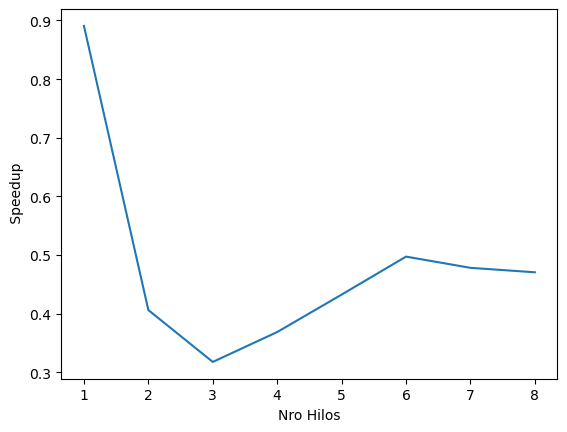
\includegraphics[scale=0.65]{./images/comparacion_speedup.png}
\end{figure}

\begin{figure}[h]
\caption{Variacion de la Eficiencia}
\centering
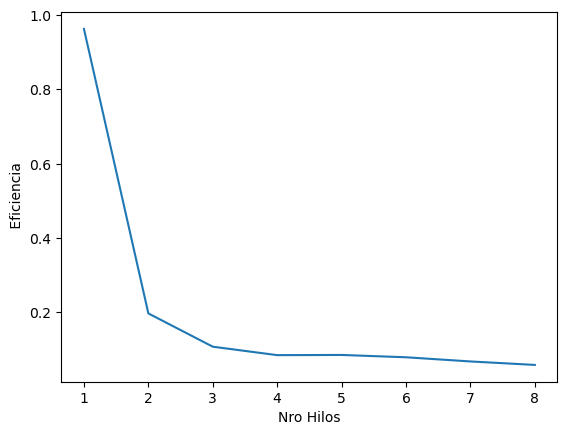
\includegraphics[scale=0.65]{./images/comparacion_efficiency.png}
\end{figure}

